\documentclass{standalone}
\usepackage{graphicx}	
\usepackage{amssymb, amsmath}
\usepackage{color}
\usepackage{wasysym}

\usepackage{tikz}
\usetikzlibrary{intersections, backgrounds}
\usepackage{pgfmath}

\definecolor{light}{RGB}{220, 188, 188}
\definecolor{mid}{RGB}{185, 124, 124}
\definecolor{dark}{RGB}{143, 39, 39}
\definecolor{highlight}{RGB}{180, 31, 180}
\definecolor{gray10}{gray}{0.1}
\definecolor{gray20}{gray}{0.2}
\definecolor{gray30}{gray}{0.3}
\definecolor{gray40}{gray}{0.4}
\definecolor{gray60}{gray}{0.6}
\definecolor{gray70}{gray}{0.7}
\definecolor{gray80}{gray}{0.8}
\definecolor{gray90}{gray}{0.9}
\definecolor{gray95}{gray}{0.95}

\newcommand*{\offset}{0.025}

\begin{document}

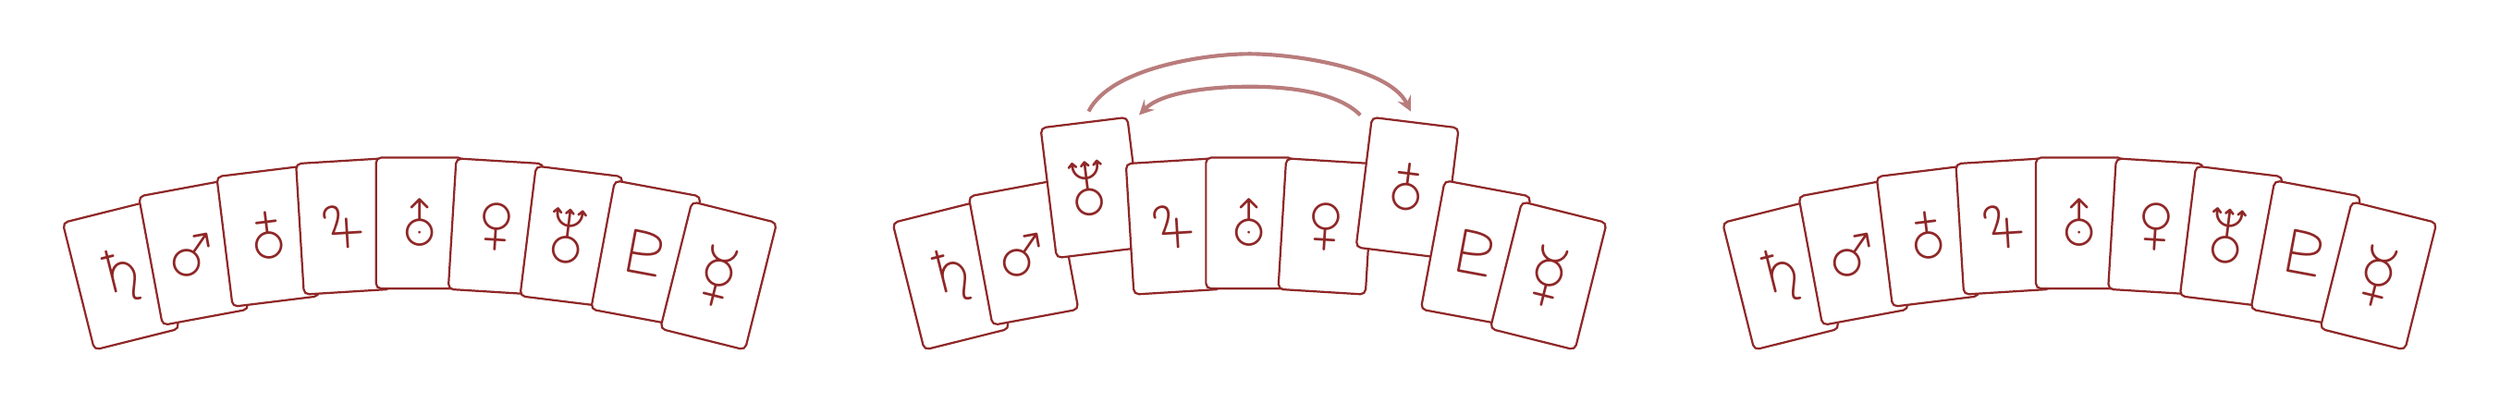
\begin{tikzpicture}[scale=0.3, thick]

% Left
\begin{scope}[shift={(-38, 0)}]

\draw[white] (-18, -7) rectangle (18, 9);

\pgfmathsetmacro{\R}{40}
\pgfmathsetmacro{\dtheta}{5}
\pgfmathsetmacro{\dphi}{3.5}

\pgfmathsetmacro{\cx}{2}
\pgfmathsetmacro{\cy}{3}

\pgfmathsetmacro{\n}{4}
\pgfmathsetmacro{\x}{\R * cos(90 + \n * \dtheta)}
\pgfmathsetmacro{\y}{\R * sin(90 + \n * \dtheta) - \R}
\begin{scope}[shift={(\x, \y)}, rotate={\dphi * \n}]
  \filldraw[fill=white, draw=dark, rounded corners=2] (0 - \cx, 0 - \cy) rectangle (0 + \cx, 0 + \cy);
  \node[dark, rotate={\dphi * \n}] at (0, 0) { $\Huge \saturn$ };
\end{scope}

\pgfmathsetmacro{\n}{3}
\pgfmathsetmacro{\x}{\R * cos(90 + \n * \dtheta)}
\pgfmathsetmacro{\y}{\R * sin(90 + \n * \dtheta) - \R}
\begin{scope}[shift={(\x, \y)}, rotate={\dphi * \n}]
  \filldraw[fill=white, draw=dark, rounded corners=2] (0 - \cx, 0 - \cy) rectangle (0 + \cx, 0 + \cy);
  \node[dark, rotate={\dphi * \n}] at (0, 0) { $\Huge \mars$ };
\end{scope}

\pgfmathsetmacro{\n}{2}
\pgfmathsetmacro{\x}{\R * cos(90 + \n * \dtheta)}
\pgfmathsetmacro{\y}{\R * sin(90 + \n * \dtheta) - \R}
\begin{scope}[shift={(\x, \y)}, rotate={\dphi * \n}]
  \filldraw[fill=white, draw=dark, rounded corners=2] (0 - \cx, 0 - \cy) rectangle (0 + \cx, 0 + \cy); 
  \node[dark, rotate={\dphi * \n}] at (0, 0) { $\Huge \earth$ };
\end{scope}

\pgfmathsetmacro{\n}{1}
\pgfmathsetmacro{\x}{\R * cos(90 + \n * \dtheta)}
\pgfmathsetmacro{\y}{\R * sin(90 + \n * \dtheta) - \R}
\begin{scope}[shift={(\x, \y)}, rotate={\dphi * \n}]
  \filldraw[fill=white, draw=dark, rounded corners=2] (0 - \cx, 0 - \cy) rectangle (0 + \cx, 0 + \cy);
  \node[dark, rotate={\dphi * \n}] at (0, 0) { $\Huge \jupiter$ };
\end{scope}

\pgfmathsetmacro{\n}{0}
\pgfmathsetmacro{\x}{\R * cos(90 + \n * \dtheta)}
\pgfmathsetmacro{\y}{\R * sin(90 + \n * \dtheta) - \R}
\begin{scope}[shift={(\x, \y)}, rotate={\dphi * \n}]
  \filldraw[fill=white, draw=dark, rounded corners=2] (0 - \cx, 0 - \cy) rectangle (0 + \cx, 0 + \cy);
  \node[dark, rotate={\dphi * \n}] at (0, 0) { $\Huge \uranus$ };
\end{scope}

\pgfmathsetmacro{\n}{-1}
\pgfmathsetmacro{\x}{\R * cos(90 + \n * \dtheta)}
\pgfmathsetmacro{\y}{\R * sin(90 + \n * \dtheta) - \R}
\begin{scope}[shift={(\x, \y)}, rotate={\dphi * \n}]
  \filldraw[fill=white, draw=dark, rounded corners=2] (0 - \cx, 0 - \cy) rectangle (0 + \cx, 0 + \cy);
  \node[dark, rotate={\dphi * \n}] at (0, 0) { $\Huge \venus$ };
\end{scope}

\pgfmathsetmacro{\n}{-2}
\pgfmathsetmacro{\x}{\R * cos(90 + \n * \dtheta)}
\pgfmathsetmacro{\y}{\R * sin(90 + \n * \dtheta) - \R}
\begin{scope}[shift={(\x, \y)}, rotate={\dphi * \n}]
  \filldraw[fill=white, draw=dark, rounded corners=2] (0 - \cx, 0 - \cy) rectangle (0 + \cx, 0 + \cy);  
  \node[dark, rotate={\dphi * \n}] at (0, 0) { $\Huge \neptune$ }; 
\end{scope}

\pgfmathsetmacro{\n}{-3}
\pgfmathsetmacro{\x}{\R * cos(90 + \n * \dtheta)}
\pgfmathsetmacro{\y}{\R * sin(90 + \n * \dtheta) - \R}
\begin{scope}[shift={(\x, \y)}, rotate={\dphi * \n}]
  \filldraw[fill=white, draw=dark, rounded corners=2] (0 - \cx, 0 - \cy) rectangle (0 + \cx, 0 + \cy);
  \node[dark, rotate={\dphi * \n}] at (0, 0) { $\Huge \pluto$ };
\end{scope}

\pgfmathsetmacro{\n}{-4}
\pgfmathsetmacro{\x}{\R * cos(90 + \n * \dtheta)}
\pgfmathsetmacro{\y}{\R * sin(90 + \n * \dtheta) - \R}
\begin{scope}[shift={(\x, \y)}, rotate={\dphi * \n}]
  \filldraw[fill=white, draw=dark, rounded corners=2] (0 - \cx, 0 - \cy) rectangle (0 + \cx, 0 + \cy);
  \node[dark, rotate={\dphi * \n}] at (0, 0) { $\Huge \mercury$ };
\end{scope}
\end{scope}

%Middle
\begin{scope}[shift={(0, 0)}]

\draw[white] (-18, -7) rectangle (18, 9);

\pgfmathsetmacro{\R}{40}
\pgfmathsetmacro{\dtheta}{5}
\pgfmathsetmacro{\dphi}{3.5}

\pgfmathsetmacro{\cx}{2}
\pgfmathsetmacro{\cy}{3}

\pgfmathsetmacro{\n}{4}
\pgfmathsetmacro{\x}{\R * cos(90 + \n * \dtheta)}
\pgfmathsetmacro{\y}{\R * sin(90 + \n * \dtheta) - \R}
\begin{scope}[shift={(\x, \y)}, rotate={\dphi * \n}]
  \filldraw[fill=white, draw=dark, rounded corners=2] (0 - \cx, 0 - \cy) rectangle (0 + \cx, 0 + \cy);
  \node[dark, rotate={\dphi * \n}] at (0, 0) { $\Huge \saturn$ };
\end{scope}

\pgfmathsetmacro{\n}{3}
\pgfmathsetmacro{\x}{\R * cos(90 + \n * \dtheta)}
\pgfmathsetmacro{\y}{\R * sin(90 + \n * \dtheta) - \R}
\begin{scope}[shift={(\x, \y)}, rotate={\dphi * \n}]
  \filldraw[fill=white, draw=dark, rounded corners=2] (0 - \cx, 0 - \cy) rectangle (0 + \cx, 0 + \cy);
  \node[dark, rotate={\dphi * \n}] at (0, 0) { $\Huge \mars$ };
\end{scope}

\pgfmathsetmacro{\n}{2}
\pgfmathsetmacro{\x}{\R * cos(90 + \n * \dtheta)}
\pgfmathsetmacro{\y}{\R * sin(90 + \n * \dtheta) - \R}
\begin{scope}[shift={(\x, \y)}, rotate={\dphi * \n}]
  \filldraw[fill=white, draw=dark, rounded corners=2] (0 - \cx, 0 - \cy + 0.75 * \cy) rectangle (0 + \cx, 0 + \cy + 0.75 * \cy); 
  \node[dark, rotate={\dphi * \n}] at (0, 0.75 * \cy) { $\Huge \neptune$ }; 
\end{scope}

\pgfmathsetmacro{\n}{1}
\pgfmathsetmacro{\x}{\R * cos(90 + \n * \dtheta)}
\pgfmathsetmacro{\y}{\R * sin(90 + \n * \dtheta) - \R}
\begin{scope}[shift={(\x, \y)}, rotate={\dphi * \n}]
  \filldraw[fill=white, draw=dark, rounded corners=2] (0 - \cx, 0 - \cy) rectangle (0 + \cx, 0 + \cy);
  \node[dark, rotate={\dphi * \n}] at (0, 0) { $\Huge \jupiter$ };
\end{scope}

\pgfmathsetmacro{\n}{0}
\pgfmathsetmacro{\x}{\R * cos(90 + \n * \dtheta)}
\pgfmathsetmacro{\y}{\R * sin(90 + \n * \dtheta) - \R}
\begin{scope}[shift={(\x, \y)}, rotate={\dphi * \n}]
  \filldraw[fill=white, draw=dark, rounded corners=2] (0 - \cx, 0 - \cy) rectangle (0 + \cx, 0 + \cy);
  \node[dark, rotate={\dphi * \n}] at (0, 0) { $\Huge \uranus$ };
\end{scope}

\pgfmathsetmacro{\n}{-1}
\pgfmathsetmacro{\x}{\R * cos(90 + \n * \dtheta)}
\pgfmathsetmacro{\y}{\R * sin(90 + \n * \dtheta) - \R}
\begin{scope}[shift={(\x, \y)}, rotate={\dphi * \n}]
  \filldraw[fill=white, draw=dark, rounded corners=2] (0 - \cx, 0 - \cy) rectangle (0 + \cx, 0 + \cy);
  \node[dark, rotate={\dphi * \n}] at (0, 0) { $\Huge \venus$ };
\end{scope}

\pgfmathsetmacro{\n}{-2}
\pgfmathsetmacro{\x}{\R * cos(90 + \n * \dtheta)}
\pgfmathsetmacro{\y}{\R * sin(90 + \n * \dtheta) - \R}
\begin{scope}[shift={(\x, \y)}, rotate={\dphi * \n}]
  \filldraw[fill=white, draw=dark, rounded corners=2] (0 - \cx, 0 - \cy + 0.75 * \cy) rectangle (0 + \cx, 0 + \cy + 0.75 * \cy);  
  \node[dark, rotate={\dphi * \n}] at (0, 0.75 * \cy) { $\Huge \earth$ };
\end{scope}

\pgfmathsetmacro{\n}{-3}
\pgfmathsetmacro{\x}{\R * cos(90 + \n * \dtheta)}
\pgfmathsetmacro{\y}{\R * sin(90 + \n * \dtheta) - \R}
\begin{scope}[shift={(\x, \y)}, rotate={\dphi * \n}]
  \filldraw[fill=white, draw=dark, rounded corners=2] (0 - \cx, 0 - \cy) rectangle (0 + \cx, 0 + \cy);
  \node[dark, rotate={\dphi * \n}] at (0, 0) { $\Huge \pluto$ };
\end{scope}

\pgfmathsetmacro{\n}{-4}
\pgfmathsetmacro{\x}{\R * cos(90 + \n * \dtheta)}
\pgfmathsetmacro{\y}{\R * sin(90 + \n * \dtheta) - \R}
\begin{scope}[shift={(\x, \y)}, rotate={\dphi * \n}]
  \filldraw[fill=white, draw=dark, rounded corners=2] (0 - \cx, 0 - \cy) rectangle (0 + \cx, 0 + \cy);
  \node[dark, rotate={\dphi * \n}] at (0, 0) { $\Huge \mercury$ };
\end{scope}

\pgfmathsetmacro{\xa}{\R * cos(90 + 2 * \dtheta) - 3.5 * sin(\dphi * 2}
\pgfmathsetmacro{\ya}{\R * sin(90 + 2 * \dtheta) - \R + 3.5 * cos(\dphi * 2)}
\pgfmathsetmacro{\xb}{\R * cos(90 - 2 * \dtheta) - 3.5 * sin(\dphi * -2)}
\pgfmathsetmacro{\yb}{\R * sin(90 - 2 * \dtheta) - \R + 3.5 * cos(\dphi * -2)}

\begin{scope}[shift={(0, 2.25)}]
  \draw[->, >=stealth, color=mid, line width=1.5] 
      (\xa, \ya) .. controls ({\xa + 1}, {\ya + 2}) and (-2, 5.5) .. (0, 5.5) .. controls (2, 5.5) and ({\xb - 1}, {\yb + 2}) ..
      (\xb, \yb);
\end{scope}

\pgfmathsetmacro{\xa}{\R * cos(90 + 1.35 * \dtheta) - 3.0 * sin(\dphi * 2}
\pgfmathsetmacro{\ya}{\R * sin(90 + 1.35 * \dtheta) - \R + 3.0 * cos(\dphi * 2)}
\pgfmathsetmacro{\xb}{\R * cos(90 - 1.35 * \dtheta) - 3.0 * sin(\dphi * -2)}
\pgfmathsetmacro{\yb}{\R * sin(90 - 1.35 * \dtheta) - \R + 3.0 * cos(\dphi * -2)}

\begin{scope}[shift={(0, 2.25)}]
  \draw[<-, >=stealth, color=mid, line width=1.5] 
      (\xa, \ya) .. controls ({\xa + 1}, {\ya + 1}) and (-2, 4) .. (0, 4) .. controls (2, 4) and ({\xb - 1}, {\yb + 1}) ..
      (\xb, \yb);
\end{scope}

\end{scope}

% Right
\begin{scope}[shift={(38, 0)}]

\draw[white] (-18, -7) rectangle (18, 9);

\pgfmathsetmacro{\R}{40}
\pgfmathsetmacro{\dtheta}{5}
\pgfmathsetmacro{\dphi}{3.5}

\pgfmathsetmacro{\cx}{2}
\pgfmathsetmacro{\cy}{3}

\pgfmathsetmacro{\n}{4}
\pgfmathsetmacro{\x}{\R * cos(90 + \n * \dtheta)}
\pgfmathsetmacro{\y}{\R * sin(90 + \n * \dtheta) - \R}
\begin{scope}[shift={(\x, \y)}, rotate={\dphi * \n}]
  \filldraw[fill=white, draw=dark, rounded corners=2] (0 - \cx, 0 - \cy) rectangle (0 + \cx, 0 + \cy);
  \node[dark, rotate={\dphi * \n}] at (0, 0) { $\Huge \saturn$ };
\end{scope}

\pgfmathsetmacro{\n}{3}
\pgfmathsetmacro{\x}{\R * cos(90 + \n * \dtheta)}
\pgfmathsetmacro{\y}{\R * sin(90 + \n * \dtheta) - \R}
\begin{scope}[shift={(\x, \y)}, rotate={\dphi * \n}]
  \filldraw[fill=white, draw=dark, rounded corners=2] (0 - \cx, 0 - \cy) rectangle (0 + \cx, 0 + \cy);
  \node[dark, rotate={\dphi * \n}] at (0, 0) { $\Huge \mars$ };
\end{scope}

\pgfmathsetmacro{\n}{2}
\pgfmathsetmacro{\x}{\R * cos(90 + \n * \dtheta)}
\pgfmathsetmacro{\y}{\R * sin(90 + \n * \dtheta) - \R}
\begin{scope}[shift={(\x, \y)}, rotate={\dphi * \n}]
  \filldraw[fill=white, draw=dark, rounded corners=2] (0 - \cx, 0 - \cy) rectangle (0 + \cx, 0 + \cy); 
  \node[dark, rotate={\dphi * \n}] at (0, 0) { $\Huge \earth$ };
\end{scope}

\pgfmathsetmacro{\n}{1}
\pgfmathsetmacro{\x}{\R * cos(90 + \n * \dtheta)}
\pgfmathsetmacro{\y}{\R * sin(90 + \n * \dtheta) - \R}
\begin{scope}[shift={(\x, \y)}, rotate={\dphi * \n}]
  \filldraw[fill=white, draw=dark, rounded corners=2] (0 - \cx, 0 - \cy) rectangle (0 + \cx, 0 + \cy);
  \node[dark, rotate={\dphi * \n}] at (0, 0) { $\Huge \jupiter$ };
\end{scope}

\pgfmathsetmacro{\n}{0}
\pgfmathsetmacro{\x}{\R * cos(90 + \n * \dtheta)}
\pgfmathsetmacro{\y}{\R * sin(90 + \n * \dtheta) - \R}
\begin{scope}[shift={(\x, \y)}, rotate={\dphi * \n}]
  \filldraw[fill=white, draw=dark, rounded corners=2] (0 - \cx, 0 - \cy) rectangle (0 + \cx, 0 + \cy);
  \node[dark, rotate={\dphi * \n}] at (0, 0) { $\Huge \uranus$ };
\end{scope}

\pgfmathsetmacro{\n}{-1}
\pgfmathsetmacro{\x}{\R * cos(90 + \n * \dtheta)}
\pgfmathsetmacro{\y}{\R * sin(90 + \n * \dtheta) - \R}
\begin{scope}[shift={(\x, \y)}, rotate={\dphi * \n}]
  \filldraw[fill=white, draw=dark, rounded corners=2] (0 - \cx, 0 - \cy) rectangle (0 + \cx, 0 + \cy);
  \node[dark, rotate={\dphi * \n}] at (0, 0) { $\Huge \venus$ };
\end{scope}

\pgfmathsetmacro{\n}{-2}
\pgfmathsetmacro{\x}{\R * cos(90 + \n * \dtheta)}
\pgfmathsetmacro{\y}{\R * sin(90 + \n * \dtheta) - \R}
\begin{scope}[shift={(\x, \y)}, rotate={\dphi * \n}]
  \filldraw[fill=white, draw=dark, rounded corners=2] (0 - \cx, 0 - \cy) rectangle (0 + \cx, 0 + \cy);  
  \node[dark, rotate={\dphi * \n}] at (0, 0) { $\Huge \neptune$ }; 
\end{scope}

\pgfmathsetmacro{\n}{-3}
\pgfmathsetmacro{\x}{\R * cos(90 + \n * \dtheta)}
\pgfmathsetmacro{\y}{\R * sin(90 + \n * \dtheta) - \R}
\begin{scope}[shift={(\x, \y)}, rotate={\dphi * \n}]
  \filldraw[fill=white, draw=dark, rounded corners=2] (0 - \cx, 0 - \cy) rectangle (0 + \cx, 0 + \cy);
  \node[dark, rotate={\dphi * \n}] at (0, 0) { $\Huge \pluto$ };
\end{scope}

\pgfmathsetmacro{\n}{-4}
\pgfmathsetmacro{\x}{\R * cos(90 + \n * \dtheta)}
\pgfmathsetmacro{\y}{\R * sin(90 + \n * \dtheta) - \R}
\begin{scope}[shift={(\x, \y)}, rotate={\dphi * \n}]
  \filldraw[fill=white, draw=dark, rounded corners=2] (0 - \cx, 0 - \cy) rectangle (0 + \cx, 0 + \cy);
  \node[dark, rotate={\dphi * \n}] at (0, 0) { $\Huge \mercury$ };
\end{scope}

\end{scope}

\end{tikzpicture}

\end{document}  